\section{Approach}

The ultimate goal of this project is to infer invariants in a
distributed system. For the scope of this project we will consider a system with 2 nodes. Before inferring invariants we need to identify likely distributed
state variables. We define distributed state variables, as variables
that are stored in one node whose values are affected or determined by
the other remote node in the distributed system. It should be noted that
these variables are only a part of the state in a distributed system
at a given time. For our case we assume that these capture a
significant portion of the state. Consider the code samples
Listing~\ref{lst:node0} and Listing~\ref{lst:node1} showing the
communication between two nodes in a distributed system. The
communication between the nodes can be depicted as shown in
Figure~\ref{fig:sample_code_diag}. We need to infer the equality
between elements in each pair \texttt{(a,first),
(b,second),(sum,result)} and also the properites: \texttt{(result = a
+ b)} and \texttt{(sum = first + second)}.


\begin{figure}
  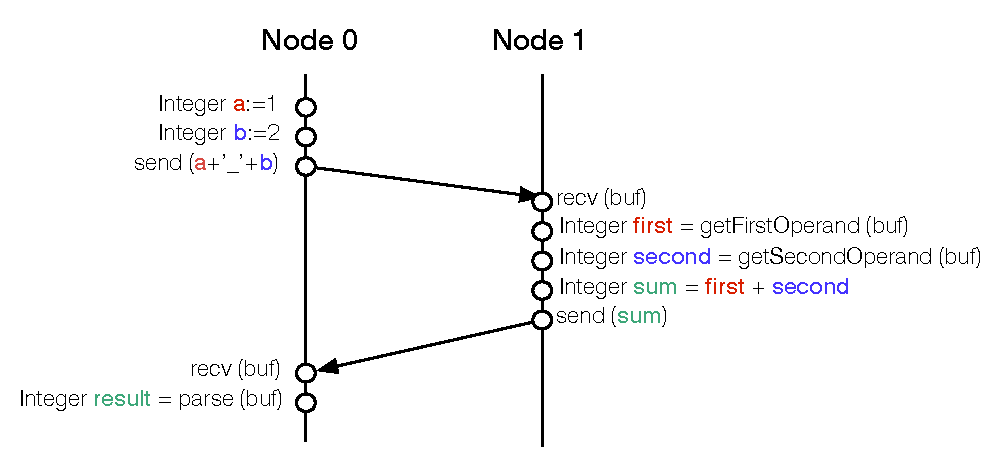
\includegraphics[width=\columnwidth]{sample_code.pdf}
  \caption{Example communication between two nodes in a distributed system}
  \label{fig:sample_code_diag}
\end{figure}

\begin{figure}
\begin{lstlisting}[caption={Sample code for Communication between 2 nodes - Node 0}, label=lst:node0]
    Integer a := 1
    Integer b := 2
    send ( a + '_' + b )
    recv (buf)
    Integer result := parse (buf)
\end{lstlisting}
\end{figure}

\begin{figure}
\begin{lstlisting}[caption={Sample code for Communication between 2 nodes - Node 1}, label=lst:node1]
    recv (buf)
    Integer first := getFirstOperand( buf )
    Integer second := getSecondOperand( buf )
    Integer sum := first + second
    send ( sum )
\end{lstlisting}
\end{figure}

The naive approach for inferring these invariants will be to dump all
state varaible values at all program points and feed them to an
invariant detector like daikon\cite{ernst2007daikon}. But given the
number of program points and huge number of variables in a relatively
large program this approach is not scalable. So we propose 2 main
optimizations to reduce the number of program point, variable value
combinations.

\subsection{Detecting interesting program points}

Rather than dumping state at all program points we expect the
developer to mark interesting program points using annotations. The
program state will be dumped at only these annotated points. This will
also help to narrow down the focus to points that are identified by
the developer as interesting points without wasting resources
analyzing useless program points. The annotations will be identified
by the parser at the instrumentation phase and re-written to include
statements which will write the values of variable to a file when the
program reaches that point in the runtime.

\subsection{Dataflow analysis for Go programs}

Even at interesting program points, variable space that need to be
captured is very large. So only the variables that were affected by
the communication with other nodes need to be identified. To detect
these variables, some form of dataflow analysis is required. This
includes the dataflow of the distributed system as a whole and also in
a single program. But currently there are no data flow analysis
frameworks available for Go programs.

This is a challenging problem in itself because Go language has
special constructs like channels to share data between goroutines. We
are planning to do this analysis dynamically by instrumenting variable
declarations and assignments, and then collecting execution traces of
each of these statements. We have chosen this approach because it
gives information about the actual execution and therefore is more
accurate. For this we are hoping to use static analysis libraries
available under Go-lang tools\cite{static_golang} which provide
support for Identifier resolution, Type information, Call graph
navigation and Channel peers (send $\leftrightarrow$ receive)
identification.

Our dynamic dataflow analysis is focused on mainly providing the
following features. Given a variable, start line and end line it will
return a set of variables affected by that variable between start line
and the end line.

As the next phase of our project, using the above analysis, we hope to
find out variables affected by receiving messages in interprocess
communication channels like RPC and TCP/UDP sockets. We will get the
values of these variables just before another send/receive or end of
function whichever occurs first. We assume these set of variables at
the send statement in both (sending and receiving) nodes taken
together represent global state of the distributed system.

Given two nodes which are communicating we have two such sets of
variables representing a particular state. So we will select the
corresponding variable pairs from send and receive of each node
mentioned in the previous step and provide as inputs for the Daikon
invariant detector. This will give us a set of properties that were
true over the observed executions across 2 nodes. Overall execution
flow of the analysis is shown in Figure~\ref{fig:go_flow}.


\begin{figure}
  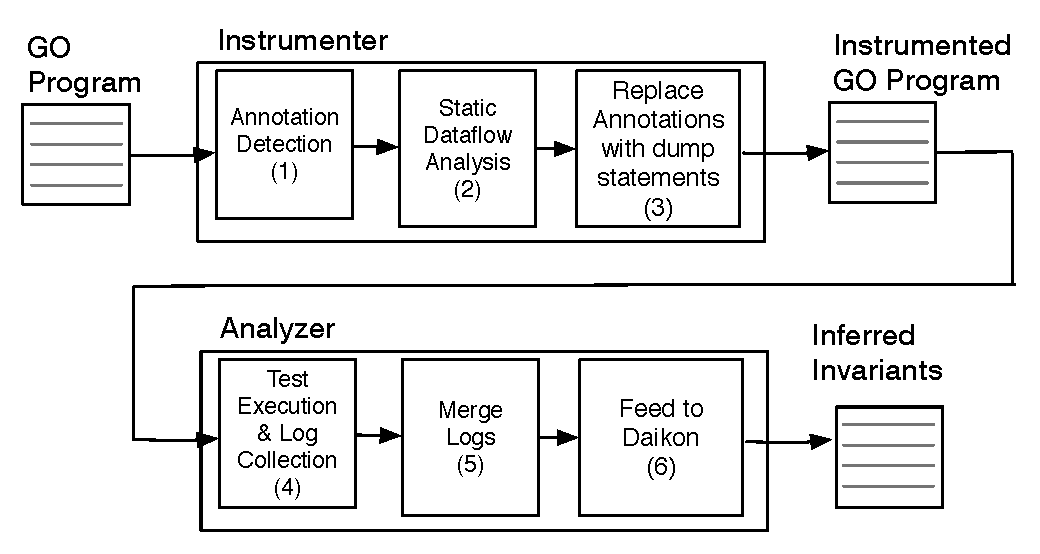
\includegraphics[width=\columnwidth]{go_flow.pdf}
  \caption{Flow of the invariant inference of Go programs}
  \label{fig:go_flow}
\end{figure}